\documentclass[12pt]{article}
 
\usepackage[utf8]{inputenc}
\usepackage[T1]{fontenc}
\usepackage{textcomp}
\usepackage[english]{babel}
\usepackage{amsmath, amssymb}
\usepackage[mathscr]{euscript}
\usepackage{subcaption}
\usepackage[margin=0.8in]{geometry}
\usepackage{graphicx}
\newtheorem{theorem}{Theorem}[section]
\newtheorem{lemma}[theorem]{Lemma}
\newtheorem{proposition}[theorem]{Proposition}
\newtheorem{corollary}[theorem]{Corollary}
\usepackage{tikz}
\usepackage{hyperref}
\hypersetup{
	colorlinks=true,
        linkcolor=blue,
        filecolor=magenta,
        urlcolor=cyan,
}
\urlstyle{same}

\newcommand{\N}{\mathbb{N}}
\newcommand{\Z}{\mathbb{Z}}
\newcommand{\Q}{\mathbb{Q}}
\newcommand{\R}{\mathbb{R}}
\newcommand{\C}{\mathbb{C}}
\newcommand{\f}{\mathfrak{f}}
\newcommand{\F}{\mathbb{F}}
\newcommand{\g}{\mathfrak{g}}
\newcommand{\K}{\mathbb{K}}
\renewcommand{\l}{\mathfrak{l}}
\newcommand{\p}{\mathfrak{p}}
\renewcommand{\P}{\mathfrak{P}}
\newcommand{\PP}{\mathbb{P}}
\newcommand\preceqdot{\mathrel{\ooalign{$\preceq$\cr
  \hidewidth\raise0.225ex\hbox{$\cdot\mkern0.5mu$}\cr}}}


\newenvironment{proof}[1][Proof]{\begin{trivlist}
\item[\hskip \labelsep {\bfseries #1}]}{\end{trivlist}}
\newenvironment{definition}[1][Definition]{\begin{trivlist}
\item[\hskip \labelsep {\bfseries #1}]}{\end{trivlist}}
\newenvironment{example}[1][Example]{\begin{trivlist}
\item[\hskip \labelsep {\bfseries #1}]}{\end{trivlist}}
\newenvironment{remark}[1][Remark]{\begin{trivlist}
\item[\hskip \labelsep {\bfseries #1}]}{\end{trivlist}}

\newcommand{\qed}{\nobreak \ifvmode \relax \else
      \ifdim\lastskip<1.5em \hskip-\lastskip
      \hskip1.5em plus0em minus0.5em \fi \nobreak
      \vrule height0.75em width0.5em depth0.25em\fi}

% figure support
\usepackage{import}
\usepackage{xifthen}
\pdfminorversion=7
\usepackage{pdfpages}
\usepackage{transparent}
\newcommand{\incfig}[1]{%
\def\svgwidth{\columnwidth}
\import{./figures/}{#1.pdf_tex}
}


\pdfsuppresswarningpagegroup=1

\begin{document}
\begin{center}
\Huge{\boldmath{Combinatorics Assignment 9}}
\end{center}
Name: Sam Laing\\
Student Number: 17323181\\
Course: Maths (JS)\\
Collaborators: none\\
References: \href{https://www.cis.upenn.edu/~cis610/sp06stanley.pdf}{Hyperplane arrangements} by Stanley, \href{https://www.ams.org/journals/bull/1999-36-02/S0273-0979-99-00775-2/S0273-0979-99-00775-2.pdf}{this article} on Hyperplane arrangements, Bona textbook.
\tableofcontents
\newpage
\section{Introduction}
We describe some basic combinatorial properties of the hyperplane arrangement $\mathcal{A}$ consisting of the hyperplanes (lines) $x=0,x=1,y=0,y=1,x+y=0$ (where $r\in \R$ is an arbitrary constant) in two-dimensional Euclidean space $V = \R^2$.\\
In particular we aim to classify the number of regions and the number of relatively bounded regions $\mathcal{A}$ divides $\R^2$ into as the parameter $r\in \R$ varies.\\
For notational simplicity, we will denote, when convenient, each of the hyperplanes as follows: \\
$H_a: x=0$, $H_b: x=1$, $H_c: y=0$, $H_d: y=1$, $H_e: x+y=r$ (or when easier just by $a,\ldots,e$)
\begin{remark}
We immediately see that for all $r\in \R$, the rank of $\mathcal{A}$ is two (since $\mathcal{A}\setminus \{H_e\} $ has 2 orthogonal and thus linearly independent normals). It then immediately follows that $\mathcal{A}$ is an essential arrangement for any chosen value of $r\in \R$.
\end{remark}
In this article we will only illustrate $\mathcal{A}$ for values of $r\in \R_{\ge 1}$ since the properties of $\mathcal{A}$ for $r\in \R_{<1}$ can be easily determined by leveraging symmetry about $y=-x+1$. When appropriate we will generalise our arguments to apply to all $r\in \R$\\
Below are illustrations of the arrangement for some values of $r\in \R_{\ge 1}$ (resp. $1,1.5,2,2.5$)
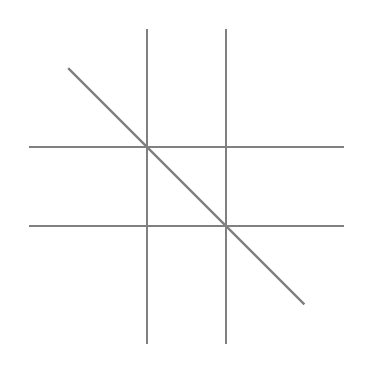
\begin{tikzpicture}
	\draw[gray,thick] (2.5,0) -- (-1.5,0);
	\draw[gray,thick] (2.5,1) -- (-1.5,1);
	\draw[gray,thick] (0,2.5) -- (0,-1.5);
	\draw[gray,thick] (1,2.5) -- (1,-1.5);
	\draw[gray,thick] (-1,2) -- (2,-1);	
\end{tikzpicture}
\hspace{0.5cm}
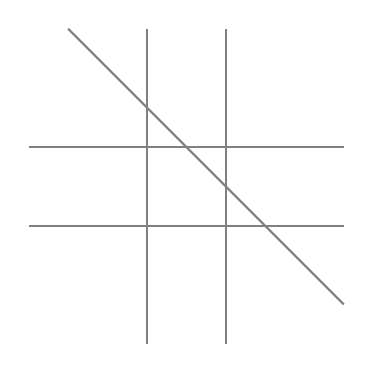
\begin{tikzpicture}
	\draw[gray,thick] (2.5,0) -- (-1.5,0);
	\draw[gray,thick] (2.5,1) -- (-1.5,1);
	\draw[gray,thick] (0,2.5) -- (0,-1.5);
	\draw[gray,thick] (1,2.5) -- (1,-1.5);
	\draw[gray,thick] (-1,2.5) -- (2.5,-1);	
\end{tikzpicture}
\hspace{0.5cm}
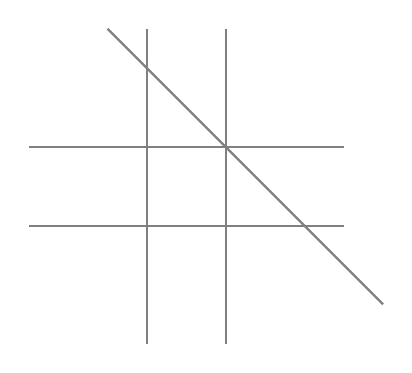
\begin{tikzpicture}
	\draw[gray,thick] (2.5,0) -- (-1.5,0);
	\draw[gray,thick] (2.5,1) -- (-1.5,1);
	\draw[gray,thick] (0,2.5) -- (0,-1.5);
	\draw[gray,thick] (1,2.5) -- (1,-1.5);
	\draw[gray,thick] (-0.5,2.5) -- (3,-1);	
\end{tikzpicture}
\hspace{0.1cm}
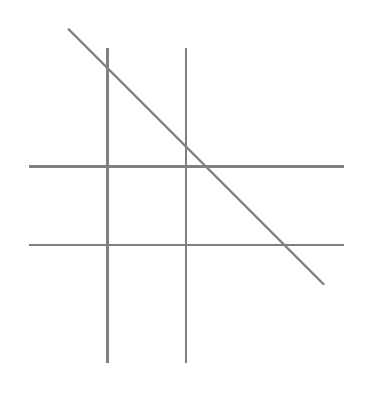
\begin{tikzpicture}
	\draw[gray,thick] (3,0) -- (-1,0);
	\draw[gray,thick] (3,1) -- (-1,1);
	\draw[gray,thick] (0,2.5) -- (0,-1.5);
	\draw[gray,thick] (1,2.5) -- (1,-1.5);
	\draw[gray,thick] (-0.5,2.75) -- (2.75,-0.5);	
\end{tikzpicture}
\newpage
\section{The Intersection Poset}
\begin{definition}
	We define the intersection poset $L(\mathcal{A})$ of a hyperplane arrangement $\mathcal{A}$ as the set of all non-empty intersections of subcollections of hyperplanes in the given arrangement (including $V=\R^{2}$): \[
		L(\mathcal{A}) := \{\bigcap_{\alpha}H_{\alpha}\neq \emptyset \mid \{H_{\alpha}\}_{\alpha}\subseteq \mathcal{A} \} 
	.\]
Equipped with the partial ordering $\preceq$ defined by: \[
	x\preceq y :\iff x \supseteq y
	.\]
\end{definition}
\begin{remark}
	For each $\alpha,\beta\in \mathcal{A}$ we denote by $\alpha\beta$ the intersection of $\alpha,\beta\in \mathcal{A}$ (i.e. $\alpha\beta := H_{\alpha}\cap H_{\beta}$)
\end{remark}
In the case of our particular arrangement ($\mathcal{A}$ ), with some help from the earlier illustrations, we consider the structure of $L(\mathcal{A})$ depending on the value of $r\in \R$:
\begin{itemize}
	\item When $r=1$ we see that $H_e$ intersects both $H_a$ and $H_d$ at the common point $(0,1)$ and intersects $H_b$ and $H_c$ at the common point $(1,0)$. There are thus 4 distinct zero-dimensional intersections for $r=1$ .
	\item Clearly choosing any two values of $r_1,r_2\in (1,2)\cup (2,+\infty)$ will result in manifestly isomorphic posets ($H_e$ will intersect each of  $H_a,\ldots,H_d$ at one distinct point none of which are equal to any intersection not involving $H_e$). In total there are $8$ distinct zero-dimensional intersections for any such $r$. Thus when considering $L(\mathcal{A})$ for values of $r\in (1,2)\cup (2,\infty)$, we are justified in considering any representative of these values. \\
		(By symmetry it is clear that in fact any value of $r\in \R\setminus\{0,1,2\}$ will yield isomorphic posets  $L(\mathcal{A})$ so there is no loss of generality)\\
We arbitrarily choose $r=\frac{3}{2}$ when appropriate but could just as well choose any $r\in \R\setminus \{0,1,2\}$ to represent.
	\item When $r=2$ we see that $H_e$ intersects $H_a$ at $ae = (0,2)$, intersects  $H_b$ and $H_d$ at the common point $bde = (1,1)$ and intersects $H_c$ at the point $ce = (0,2)$. So there are $6$ distinct zero dimensional intersections in this case (similarly by symmetry an isomorphic poset to this can be recovered by setting $r=0$ )
\end{itemize}

\begin{remark}
	These are the only possible structures for the intersection since $H_e$ must intersect all other hyperplanes and the points $(1,0)$ and $(0,1)$ are colinear in relation to $H_e$. (a more formal description is provided at the end)\\
	the two special cases are for $r=1$ and for $r\in \{0,2\}$, else the intersection poset has the same structure. 
\end{remark}
\begin{remark}
	Since the intersection of all hyperplanes in $\mathcal{A}$ is always empty (for any $r\in \R$), our arrangement is never central. As a result of this, by Proposition 2.3 of Stanley, $L(\mathcal{A})$ is never a lattice. 
\end{remark}
\newpage
\section{Hasse Diagrams for $L(\mathcal{A})$}
$L(\mathcal{A})$ has a corresponding Hasse diagram which depends on the value of $r\in \R_{\ge 1}$\\
From the illustrations (in the introduction) it is clear that the non empty intersections in $\mathcal{A}$ are $V=\R^2$ (trivially), each hyperplane (trivial one element intersection) and 0 dimensional subspaces (points) which depend on the chosen value of $r$. That is, for each $r\in \R_{\ge 1}$ the Hasse diagram of $L(\mathcal{A})$ consists of 3 "levels"\\
\\
\\
\begin{tikzpicture}
  \node (f) at (-2.5,2.5) {$ade$};
  \node (g) at (-1,2.5) {$bd$ };
  \node (h) at (1,2.5) {$ac$ };
  \node (i) at (2.5,2.5) {$bce$ };
  \node (a) at (-3,0) {$a$};
  \node (b) at (-1.5,0) {$b$};
  \node (e) at (0,0) {$e$};
  \node (c) at (1.5,0) {$c$};
  \node (d) at (3,0) {$d$ }; 
  \node (min) at (0,-2) {$V$};
  \draw (min) -- (a) -- (f) -- (e) -- (i) -- (c) -- (min)
	  (min) -- (b) -- (g) -- (d) -- (min)
	  (min) -- (e)
	  (d) -- (f)
	  (b) -- (i)
	  (c) -- (h) --(a)

\end{tikzpicture}
\hspace{1 cm}
\begin{tikzpicture}
  \node (f) at (-3.5,2.5) {$ad$};
  \node (g) at (-2.5,2.5) {$ae$ };
  \node (h) at (-1.65,2.5) {$bd$ };
  \node (i) at (-0.5,2.5) {$be$ };
  \node (j) at (0.5,2.5) {$ac$ };
  \node (k) at (1.65,2.5) {$de$ };
  \node (l) at (2.5,2.5) {$bc$ };
  \node (m) at (3.5,2.5) {$ce$ };
  \node (a) at (-3,0) {$a$};
  \node (b) at (-1.5,0) {$b$};
  \node (e) at (0,0) {$e$};
  \node (c) at (1.5,0) {$c$};
  \node (d) at (3,0) {$d$ }; 
  \node (min) at (0,-2) {$V$};
  \draw (min) -- (a) -- (f) -- (d) -- (min)
	  (a) -- (g) -- (e) -- (min) 
	  (a) -- (j) -- (c) -- (min)
	  (b) -- (i) -- (e) -- (k) -- (d)
	  (b) -- (l) -- (c)
	  (e) -- (m) -- (c)
	(min) -- (b)-- (h) -- (d) 
\end{tikzpicture}
\\

\begin{tikzpicture}
  \node (f) at (-3.5,2.5) {$ad$};
  \node (g) at (-2,2.5) {$ae$ };
  \node (h) at (-0.5,2.5) {$ac$ };
  \node (i) at (1,2.5) {$bc$ };
  \node (j) at (2.25,2.5) {$bde$ };
  \node (l) at (3.5,2.5) {$ce$ };
  \node (a) at (-3,0) {$a$};
  \node (b) at (-1.5,0) {$b$};
  \node (e) at (0,0) {$e$};
  \node (c) at (1.5,0) {$c$};
  \node (d) at (3,0) {$d$ }; 
  \node (min) at (0,-2) {$V$};
  \draw (min) -- (a) -- (g) -- (e)
	  (a) -- (f) -- (d)
	  (a) -- (h) -- (c)
	  (a) -- (g) -- (e) -- (min) 
	  (min) -- (b) -- (i) -- (c) -- (min) -- (d) -- (j) -- (e) -- (l) -- (c)
	  (b) -- (j)
\end{tikzpicture}
\begin{remark}
	Above are the Hasse diagrams representing $L(\mathcal{A})$ for $r=1,1.5,2$ respectively Indeed these are the only possible Hasse diagrams for any  $r\in \R$
\end{remark}
\begin{remark}
	We see that $L(\mathcal{A})$ is a graded poset for any $r\in \R$. We thus have an obvious corresponding rank function $rk: L(\mathcal{A}) \to \N$ where each vertex in the $i^{th}$ level of the corresponding Hasse diagram has rank $i$ (for  $i\in {0,1,2} $).\\
	For example in the first diagram we can clearly see $rk(V) = 0$, $rk(a) = 1, rk(ade) = 2$ etc.
\end{remark}
\section*{The Characteristic Polynomial}
We now use our Hasse diagrams to derive some of the defining properties of $\mathcal{A}$: \\
Firstly we compute the characteristic polynomial ($\chi_{\mathcal{A}}(t)$) of $\mathcal{A}$ in the three specified cases ($r=1,r=1.5,r=2$). We could do this using the Deletion Restriction theorem or Whitney's theorem but it seems like senseless overkill here since the Hasse diagrams make it easy to find the characteristic polynomial in each case directly from the definition (using iteration, and Theorem 16.5 from Bona, to compute $\mu (x)$) .  
\begin{itemize}
	\item If $r = 1$, we see that $\mu (V) = 1$, $\mu(x) = -1 \text{ if } x\in \{a,b,c,d,e\} $, $\mu (ade) = \mu (bce) = 2$ and $\mu (bd) = \mu (ac) = 1$. We then easily recover \[
			\chi_{\mathcal{A}}(t) = \sum_{x\in L(\mathcal{A})}^{} {\mu (x)t^{dim(x)}} = t^2-5t+6 
	.\]
\item Let $r=1.5$ (representing the class of combinatorically equivalent arrangements for  $r\in (1,2)\cup (2,\infty)$). We see then that each 0-dimensional intersection (3rd level of corresponding Hasse diagram) has degree 2 and thus $\mu (\alpha\beta) = 1$ $\forall \alpha,\beta\in L(\mathcal{A})$. We then see: \[
		\chi_{\mathcal{A}}(t) = t^2-5t+8
.\]  
(Indeed it is easy to see that this is the characteristic polynomial of $\mathcal{A}$ for any chosen value of $r\in \R\setminus\{0,1,2\}$)
	\item Let $r=2$, Just for fun let's compute the characteristic polynomial using the Deletion Restriction Theorem: Consider the distinguished hyperplane $H_e\in \mathcal{A}$ and the triple $(\mathcal{A}, \mathcal{A}', \mathcal{A}'')$. The characteristic polynomial of $\mathcal{A}' := \mathcal{A}\setminus H_e$ is clearly given by $t^2-4t+4$, \\
		$\mathcal{A}'':=\mathcal{A}^{H_e}$ (the restriction of $\mathcal{A}$ to $H_{e}$) has characteristic polynomial $t-3$ (since there are 3 intersection points on the line $H_e$). Hence by the Deletion Restriction Theorem, we have \[
			\chi_{\mathcal{A}}(t) = \chi_{\mathcal{A}'}(t) - \chi_{\mathcal{A}''}(t) = t^2-5t+7
		.\]
	We note that, again by symmetry, the characteristic polynomial for $r=0$ would be the same.
\end{itemize}
\section*{Computing $r(\mathcal{A})$ and $b(\mathcal{A})$ }
\begin{definition}
	We define:\\
	$r(\mathcal{A}) := \# (V\setminus \bigcup_{H\in \mathcal{A}}^{} H) = $ the number of regions of $\mathcal{A}$ \\
	\\
	$b(\mathcal{A}) := $ the number of relatively bounded regions in $\mathcal{A}$
\end{definition}
For each of the three possible characteristic polynomials of $\mathcal{A}$, we now apply Zaslavsky's Theorem to count both the number of regions and the number of relatively bounded regions: 
\begin{itemize}
	\item Let $r=1$, Then, by Zaslavsky's Theorem, the number of regions is given by: \[
			r(\mathcal{A}) =(-1)^2 \chi_{\mathcal{A}}(-1) = 12
	.\] 
	and the number of relatively bounded regions is given by: \[
		b(\mathcal{A}) = (-1)^2 \chi_{\mathcal{A}}(1) = 2
	.\] 
\item Now consider the case where $r=2$ (or by symmetry $r=0$).\\
	The number of regions is given by $r(\mathcal{A}) = 13$ and the number of relatively bounded regions is given by $b(\mathcal{A}) = 3$
	\item Now for any other choice of $r\in \R\setminus\{0,1,2\}$, we have the same characteristic polynomial. Thus we conclude that in any such case, the number of regions of $\mathcal{A}$ is  $14$ and the number of relatively bounded regions is $5$
\end{itemize}
\begin{remark}
	One can readily verify that these computations are correct by simply counting the number of regions and the number of relatively bounded regions on the illustrations in the introduction. 
\end{remark}
We thus conclude that the \underline{only} possible number of regions (resp. relatively bounded regions) of this arrangement are $12,13,14$ (resp. 2,3,5). The number of regions is 12 if and only if $r=1$ and the number of regions is 13 if and only if $r\in \{0,2\}$, else the arrangement has 14 regions in $\R^2$.\\
\\
More formally let $\mathcal{A}_r$ denote our hyperplane arrangement for a particular value $r\in \R$. Consider the collection of all such hyperplanes: $\{\mathcal{A}_{r}\}_{r\in \R}$. \\
One easily sees that \[
	\mathcal{A}_{r_1} \sim \mathcal{A}_{r_2} :\iff L(\mathcal{A}_{r_1}) \text{ and } L(\mathcal{A}_{r_2}) \text{ are isomorphic as posets} 
.\]  
defines an equivalence relation on our set. \\
Since the set of equivalence classes has cardinality 3 and the structure of $L(\mathcal{A})$ uniquely determines the characteristic polynomial of the arrangement, by Zalavsky's Theorem we have completely categorized the number of regions (and relatively bounded regions) of $\mathcal{A}$ for any value of $r\in \R$. So powerful results from combinatorics yield an elegant and complete solution to this ostensibly simple problem.
\end{document}
